% slides.tex
\documentclass[20pt]{beamer}
\usepackage{listings}
\usepackage[utf8]{inputenc}
\usepackage{cancel}
\usepackage{color}
\usepackage{graphicx}
\usepackage{pdfpages}
\usepackage{amsmath}
\usepackage{xcolor}

\usetheme{default}
\usecolortheme{dove}
\useoutertheme{default}

% Remove navigation symbols
\setbeamertemplate{navigation symbols}{}

% Slightly smaller title
\setbeamerfont{frametitle}{size=\large}
\setbeamerfont{verb}{size=\small}

% Font
\renewcommand{\ttdefault}{pcr}

% lst settings
\lstset{
    basicstyle=\ttfamily\footnotesize,
    gobble=4,
    keywordstyle=\ttfamily\bfseries,
    showstringspaces=false
}

\newcommand{\vspaced}{
    \vspace{5mm}
}

\newcommand{\fullimageframe}[1]{
    {
        \usebackgroundtemplate{
            \includegraphics[height=\paperheight,width=\paperwidth]{#1}}
        \setbeamertemplate{navigation symbols}{}
        \begin{frame}[plain]
        \end{frame}
    }
}

\newcommand{\imageframe}[1]{
    {
        \begin{frame}[plain]
        \begin{center}
        \includegraphics[width=\textwidth]{#1}
        \end{center}
        \end{frame}
    }
}

\newcommand{\chapterslide}[1]{
    {
        \begin{frame}[plain]
        \begin{center}
        \large{#1}
        \end{center}
        \end{frame}
    }
}

\newcommand{\code}[1]{
    \texttt{\small{#1}}
}

\definecolor{asparagus}{rgb}{0.53, 0.66, 0.42}
\definecolor{bittersweet}{rgb}{1.0, 0.44, 0.37}

\begin{document}

\title{Hakyll: \\
tutorial and internals}
\subtitle{Munihac}
\author{Jasper Van der Jeugt}
\date{September 2, 2016}

\begin{frame}[plain]
    \titlepage
\end{frame}

\begin{frame}{About me}
    \begin{itemize}
    \item I like skateboards, photography and Haskell
    \item Contributed to and authored open source projects
    \item Worked with Haskell for some companies
    \item Currently at \code{fugue.co}
    \end{itemize}
\end{frame}

\begin{frame}{About this talk}
    \begin{itemize}
    \item Static site generators?
    \item Hakyll
    \item Tutorial/demo
    \item Dependency handling
    \end{itemize}
\end{frame}

\chapterslide{Static site generators}

\begin{frame}{Static site generators}
    Back when things were simple \\
    \vspaced
    \begin{itemize}
    \item Write HTML
    \item FTP to server
    \item svn commit
    \item everyone was happy
    \item then something horrible happened
    \end{itemize}
\end{frame}

\imageframe{images/php.jpg}

\imageframe{images/cms.png}

\begin{frame}{Static site generators}
    \small{
    Ace acrylamid Blacksmith Blogofile Bonsai Cactus Chisel coleslaw
    Composer cyrax Deplot Fairytale Floyd FMPP Frank fugitive gostatic Graze
    \textbf{Hakyll} Hammer Hastie Hobix Hyde Jekyll jinjet jkl Korma Letterpress
    Machined Magneto Markbox Markdoc Middleman mynt nanoc Nikola Pagegen
    Pelican Petrify Phrozn PieCrust Pilcrow Pith poole Punch Quill...
    }
\end{frame}

\begin{frame}[fragile]{Static site generators}
    \textbf{\texttt{posts/munihac.md}}:
    \vspaced
    \begin{lstlisting}
    ---
    title: Munihac
    ---

    I am **really** looking
    forward to it.

    I should ask mom if I'm
    allowed to go.
    \end{lstlisting}
\end{frame}

\begin{frame}[fragile]{Static site generators?}
    \textbf{\texttt{templates/post.html}}:
    \vspaced
    \begin{lstlisting}[language=HTML]
    <h1>$title$</h1>
    <div class="post">
      $body$
    </div>
    \end{lstlisting}
\end{frame}

\begin{frame}[fragile]{Static site generators?}
    \textbf{\texttt{\_site/posts/munihac.html}}:
    \vspaced
    \begin{lstlisting}[language=HTML]
    <h1>Munihac</h1>
    <div>
      <p>
        I am <strong>really</strong>
        looking forward to it.
      </p>
      ...
    </div>
    \end{lstlisting}
\end{frame}

\begin{frame}{Static site generators?}
    \textbf{Advantage: super fast} \\
    \vspaced
    One \texttt{sendfile(2)} vs. a few database queries and rendering the final
    result \\
    \vspaced
    Akamai, Amazon CloudFront\ldots
\end{frame}

\begin{frame}[fragile]{Static site generators?}
    \textbf{Advantage: no vulnerabilities} \\
    \vspaced
    \begin{lstlisting}[language=bash]
    curl
      http://site.com/archive.php\
      ?query=DELETE+FROM+...
    \end{lstlisting}
\end{frame}

\begin{frame}{Static site generators?}
    \textbf{Advantage: host support} \\
    \vspaced
    \textbf{CMS:} Apache, FTP, Python, MySQL, memcached\ldots \\
    \vspaced
    \textbf{SSG:} I can probably host it on my microwave if I need to
\end{frame}

\begin{frame}[fragile]{Static site generators?}
    \textbf{Advantage: use version control} \\
    \vspaced
    \begin{lstlisting}[language=bash]
    $ git log
    72fb81 Add WebSockets blogpost
    5ebaf9 Typo fixes
    f93858 Quick CSS fix
    2913bb Update homepage
    ...
    \end{lstlisting}
\end{frame}

\begin{frame}{Static site generators?}
    \textbf{Advantage: use your favorite text editor (which is VIM)} \\
    \vspaced
    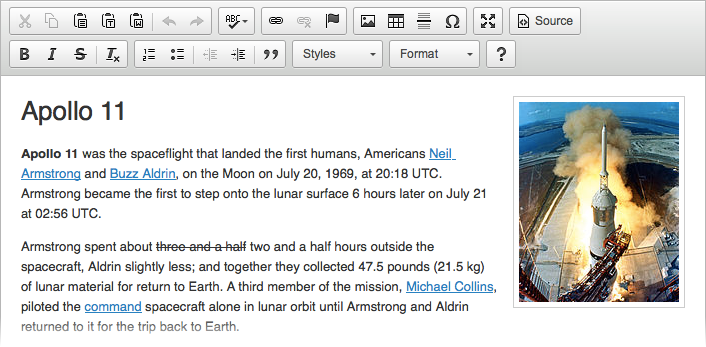
\includegraphics[width=\textwidth]{images/wysiwyg.png}
\end{frame}

\chapterslide{Hakyll}

\begin{frame}{Hakyll}
    \begin{itemize}
    \item Fairly mature (2009)
    \item Haskell, Pandoc
    \item Configuration = Code
    \item More library than application
    \end{itemize}
\end{frame}

\chapterslide{Tutorial/demo}

\chapterslide{Hakyll: Dependency handling}

\begin{frame}{Dependency handling}
    Two big questions: \\
    \vspaced
    In what order should we build items? \\
    Which items are out-of-date? \\
\end{frame}

\chapterslide{Scheduling items}

\imageframe{{images/deps-01.dot}.pdf}

\begin{frame}{Scheduling items}
    \begin{enumerate}
    \item \code{a.jpg}
    \item \code{b.jpg}
    \item \code{default.html}
    \item \code{index.html}
    \end{enumerate}
\end{frame}

\begin{frame}{Scheduling items}
    \begin{enumerate}
    \item \code{b.jpg}
    \item \code{default.html}
    \item \code{a.jpg}
    \item \code{index.html}
    \end{enumerate}
\end{frame}

\begin{frame}{Scheduling items}
    But there is no order information in the \code{site.hs}!
\end{frame}

\begin{frame}{Scheduling items}
    Early Hakyll versions: compute dependency graph \emph{before} starting to
    build.  This was based on \emph{Arrows}.
\end{frame}

\begin{frame}[fragile]{Scheduling items}
    Problem with \emph{Arrows}: \\
    \vspaced
    \begin{lstlisting}
    field "authorBio" $ \item ->
      let self = itemIdentifier item
      authorPath <-
        getMetadataField self "author"
      bio <- load
        (fromFilePath authorPath)
      ...
    \end{lstlisting}
\end{frame}

\begin{frame}{Scheduling items}
    Not requiring to compute the dependency graph before we start the build is
    \emph{way more flexible}!
\end{frame}

\begin{frame}{Compiler Monad}
    We solve this ---unsurprisingly--- by having a sort of AST and
    \emph{interpreter}.
\end{frame}

\begin{frame}[fragile]{Compiled Monad}
    \begin{lstlisting}
    data CompilerResult a
      = CompilerDone a
      | CompilerError String
      | CompilerRequire
          Identifier (Compiler a)

    newtype Compiler a = Compiler
      { unCompiler ::
          IO (CompilerResult a)
      }
    \end{lstlisting}
\end{frame}

\begin{frame}[fragile]{Compiled Monad}
    \begin{lstlisting}
    return =
      Compiler . return . CompilerDone
    Compiler c0 >>= f = Compiler $ do
      res <- c0
      case res of
        CompilerDone x ->
          unCompiler $ f x
        CompilerError e ->
          return $ CompilerError e
        CompilerRequire i c1 -> return $
          CompilerRequire i (c1 >>= f)
    \end{lstlisting}
\end{frame}

\begin{frame}[fragile]{Scheduler}
    \begin{lstlisting}
    data ScheduleState
      = Done
      | forall a. Paused (Compiler a)

    type Scheduler =
      M.Map Identifier ScheduleState

    -- Everything starts in 'Paused'...

    \end{lstlisting}
\end{frame}

\begin{frame}[fragile]{Scheduler}
    \begin{lstlisting}
    schedule
      :: Identifier -> Scheduler
      -> IO Scheduler
    schedule id0 scheduler =
      case M.lookup id0 scheduler of
        Nothing -> fail "..."
        Just Done -> return scheduler
        Just (Paused c0) -> do
          res <- unCompiler c0
          case res of
            ...
    \end{lstlisting}
\end{frame}

\begin{frame}[fragile]{Scheduler}
    \begin{lstlisting}
    case res of
      CompilerDone x -> return $
        M.insert id0 Done scheduler
      CompilerError e ->
        fail e
      CompilerRequire id1 c1 -> schedule
        id1
        (M.insert id0
          (Paused c1) scheduler)
    \end{lstlisting}
\end{frame}

\begin{frame}{Scheduler}
    Some other things: \\
    \vspaced
    Cycle detection \\
    Writing to disk and cache \\
    \ldots
\end{frame}

\chapterslide{Out-of-date items}

\begin{frame}[fragile]{Out-of-date items}
    \begin{lstlisting}
    data ScheduleState
      = Done
      | forall a. Paused (Compiler a)

    type Scheduler =
      M.Map Identifier ScheduleState

    -- Everything starts in 'Paused'...
    -- Or not...
    \end{lstlisting}
\end{frame}

\begin{frame}{Out-of-date items}
    Before we start scheduling items we have no idea what the dependency graph
    will look like. \\
    \vspaced
    But we know what it looked like for the previous run.
\end{frame}

\imageframe{{images/deps-01.dot}.pdf}
\imageframe{{images/deps-02.dot}.pdf}
\imageframe{{images/deps-03.dot}.pdf}
\imageframe{{images/deps-04.dot}.pdf}
\imageframe{{images/deps-05.dot}.pdf}
\imageframe{{images/deps-06.dot}.pdf}

\begin{frame}{Out-of-date items}
    When we build an item, we store: \\
    \vspaced
    The result, obviously \\
    The list of dependencies!
\end{frame}

\begin{frame}[fragile]{Out-of-date items}
    On re-run: \\
    \vspaced
    \begin{lstlisting}
    "index.html":
      [ "a.jpg"
      , "b.jpg"
      , "default.html"
      ]
    \end{lstlisting}
\end{frame}

\imageframe{{images/deps-04.dot}.pdf}

\begin{frame}[fragile]{Out-of-date items}
    We loaded the list using: \\
    \vspaced
    \begin{lstlisting}
    loadAll "pictures/*" >>= recentFirst
    \end{lstlisting}
\end{frame}

\begin{frame}[fragile]{Out-of-date items}
    A pattern can be considered as a \emph{predicate} on identifiers. \\
    \vspaced
    \begin{lstlisting}
    data Pattern = ...

    instance Binary Pattern -- !!!

    loadAll
      :: (Binary a, Typeable a)
      => Pattern
      -> Compiler [Item a]
    \end{lstlisting}
\end{frame}

\begin{frame}[fragile]{Out-of-date items}
    \begin{lstlisting}
    data Dependency
      = ItemDep Identifier
      -- Pattern, and result
      | PatternDep Pattern [Identifier]
    \end{lstlisting}
\end{frame}

\begin{frame}[fragile]{Out-of-date items}
    \begin{lstlisting}
    "index.html":
      [ PatternDep
          "pictures/*"
          ["a.jpg", "b.jpg"]
      , ItemDep "a.jpg"
      , ItemDep "b.jpg"
      , ItemDep "default.html"
      ]
    \end{lstlisting}
\end{frame}

\begin{frame}{Out-of-date items}
    Conclusion: we can \emph{re-evaluate} the \code{Pattern} and check the new
    result against the result from the previous run.  If there is a difference,
    the item is out-of-date.
\end{frame}

\chapterslide{Questions?}

\end{document}
